	\begin{figure}[!h]
		\centering
 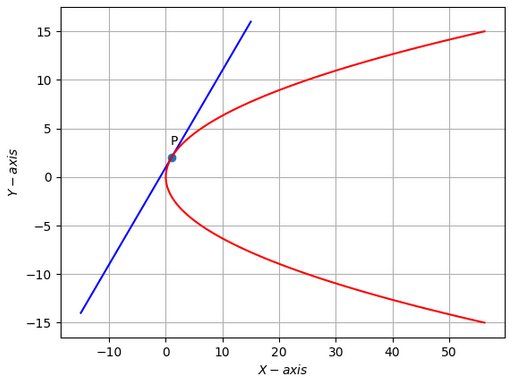
\includegraphics[width=\columnwidth]{chapters/12/6/3/27/figs/conicfig.png}
		\caption{}
		\label{fig:12/6/3/27}
  	\end{figure}
The parameters of the conic are
\begin{align}
 \vec{V} = \myvec{0&0\\0&1},  \vec{u} = \myvec{-2&0}, f = 0 
\end{align}
Following the approach in Problem 
\ref{chapters/12/6/3/15},
since
\begin{align}
	\vec{n} = \myvec{1 \\ -1}
\end{align}
we obtain
\begin{align}
	\vec{q} = \myvec{1 \\ 2}
\end{align}
See 
		\figref{fig:12/6/3/27}.

